\section{Generative Modeling}
\textbf{Goal}: \(p_{data} \sim p_{model}\)

Model the data's density distribution.
If accurate, we can sample  new points from the distribution an they will be properly correlated such that the new instance looks like it came from the data distribution.
\subsection{Overview}
\subsubsection{Probability density function}
\(p(x) \ge 0, \forall_x \in X\) Always positive 

\(\int_X p(x)dx = 1\) Probability must sum to one

Elements in the support compete in a zero sum game for probability mass density.
\subsubsection{Discriminative Model}
Learn probability distribution \(p(y|x)\)

Discriminant models.
The possible labels compete for probability mass but not the images themselves.
\begin{figure}[!h]
    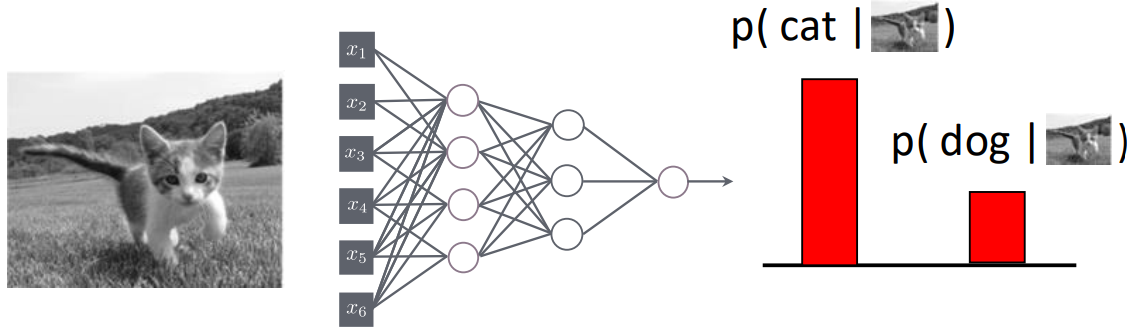
\includegraphics[width = \columnwidth]{figures/GenAI1/DiscriminativeModel.png}
\end{figure}


\subsubsection{Generative Model}
Learn a probability distribution \(p(x)\)

Generative models can reject unreasonable images by assigning them low mass.
\begin{figure}[!h]
    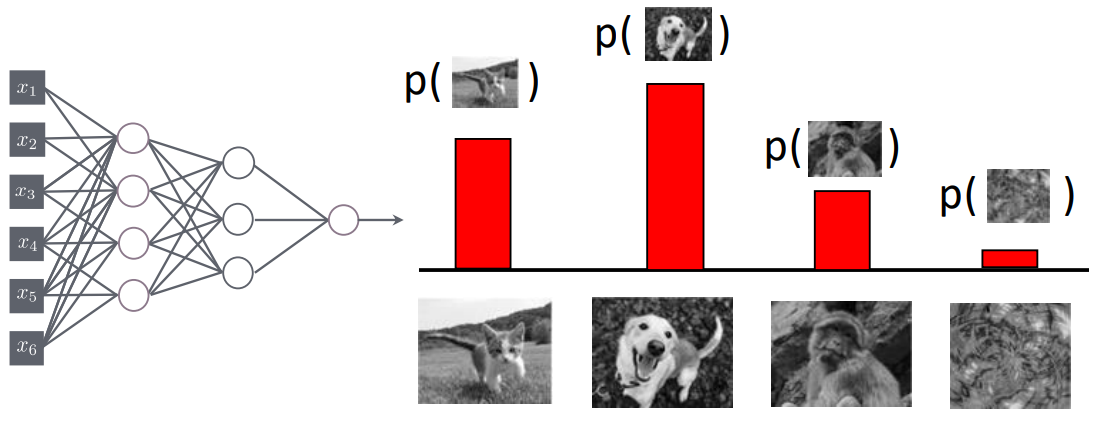
\includegraphics[width = \columnwidth]{figures/GenAI1/GenerativeModel.png}
\end{figure}

Generative models: All possible images compete against one another for probability mass.

Requires deep image understanding, is a dog more likely to sit or stand? How likely is a three legged dog?

\subsubsection{Conditional Generative Model}
Learn a probability distribution \(p(x|y)\)

\begin{figure}[!h]
    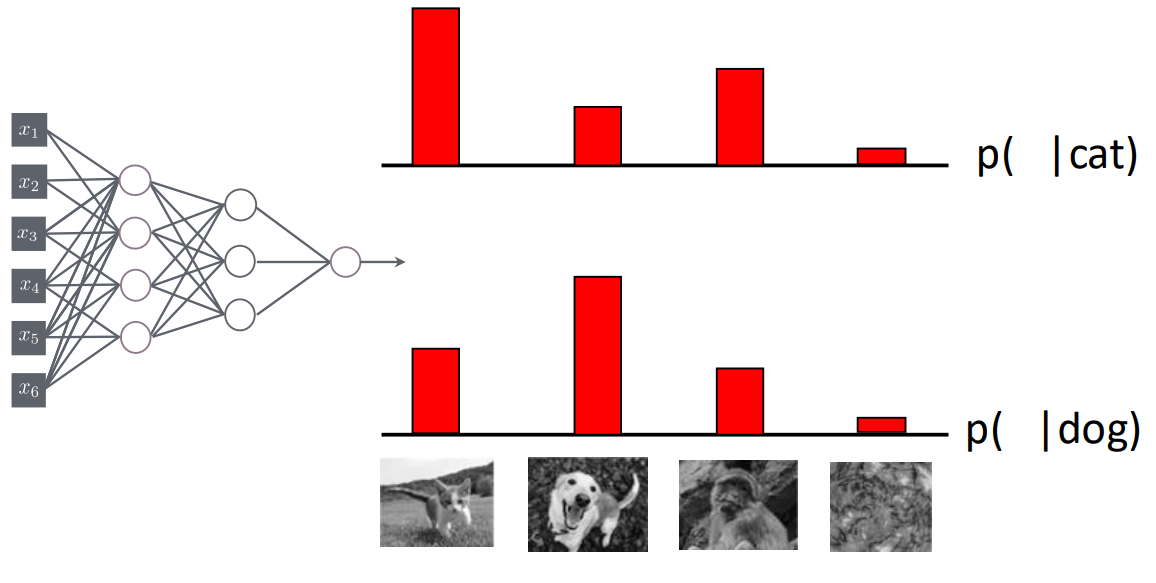
\includegraphics[width = \columnwidth]{figures/GenAI1/ConditionalGenerativeModel.png}
\end{figure}
Conditional Generative models: each label induces a competition amongst all images.

\subsubsection{Bayes formula for Generative Models}
\[
P(x|y) = \frac{P(y|x)}{P(y)}P(x)
\]

\begin{itemize}
    \item \textbf{Conditional generative model} \(P(x|y)\): Probability of the given data a certain class
    \item \textbf{Discriminant model} \(P(y|x)\):Given the data how likely is a label
    \item \textbf{Marginal probability} \(P(y)\):Frequency of occurence
    \item \textbf{Generative model} \(P(x)\): GAN, VAE, etc. 
\end{itemize}

\subsubsection{Shannon Entropy}
\[
H(p) = - \sum_x p(x) \text{log} p(x)
\]
\begin{figure}[!h]
    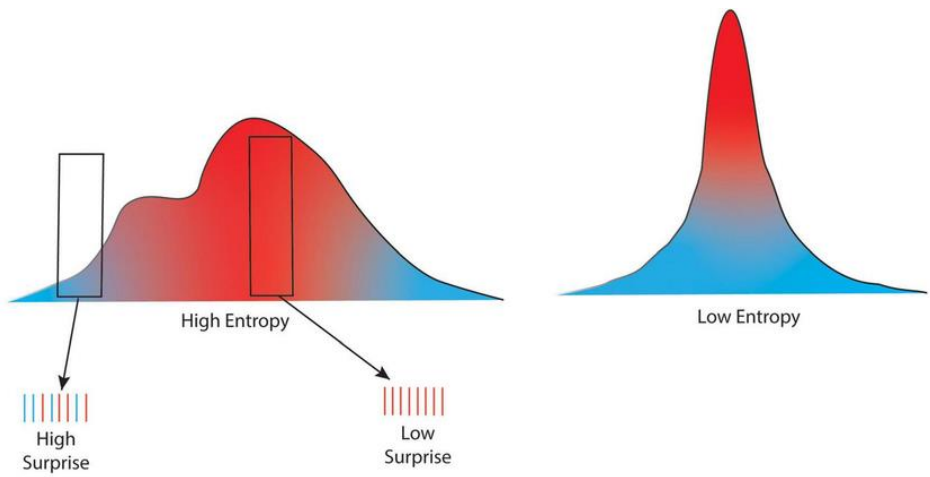
\includegraphics[width = \columnwidth]{figures/GenAI1/ShannonEntropy.png}
\end{figure}